\documentclass[polish]{beamer}

\usepackage{polski}
\usepackage{tikz}
\usepackage[beamer,customcolors]{hf-tikz}
\usepackage{nameref}
\usepackage{multicol}
\usepackage{tabu}
\usepackage{listings}
\usepackage[justification=centering]{caption}

\makeatletter
\newcommand*{\currentname}{\@currentlabelname}
\makeatother

\usetheme[titlepagelogo=images/template/Logo-PL.jpg,
  color=green,
  language=polish,
  pageofpages=z
  ]{TorinoTh}
\author{Michał Sośnicki}
\rel{dr inż. Jan Stolarek}
\title[Praca inżynierska]{Usprawnienie programowania z użyciem\\ typów w Glasgow Haskell Compiler}
\ateneo{Politechnika Łódzka}
\date{\today}

\setrellabel{Promotor}
\setcandidatelabel{Dyplomant}
\setsubject{Praca inżynierska}

\hfsetfillcolor{alerted text.fg!10}
\hfsetbordercolor{alerted text.fg}

\setbeamertemplate{section in toc}[sections numbered]
\setbeamertemplate{subsection in toc}[subsections numbered]
\setbeamertemplate{frametitle continuation}[from second]
\setbeamercolor{section in toc}{fg=alerted text.fg}
\setbeamercolor{subsection in toc}{fg=alerted text.fg}

\setbeamertemplate{bibliography item}[text]
\setbeamercolor{bibliography entry author}{fg=normal text.fg}

\setbeamercolor{caption name}{fg=normal text.fg}

\hypersetup{linkcolor=normal text.fg}

\def\figurename {Rys.}

% Usage:
% \tikzoverlay at (-1cm,-5cm) {content};
% or
% \tikzoverlay[text width=5cm] at (-1cm,-5cm) {content};
\tikzset{
  every overlay node/.style={
    %draw=black,fill=white,rounded corners,
    anchor=north west, inner sep=0pt,
  },
}

\def\tikzoverlay{%
   \tikz[remember picture, overlay]\node[every overlay node]
}%

\begin{document}

\titlepageframe

\section{Wstęp} %%%%%%
\subsection{Kompilator} %%%
\begin{frame}[t,fragile]{\currentname}
\tikzoverlay (n0) at (0cm,0cm) {%
\begin{minipage}{0.4\textwidth}%
    \begin{figure}[H]
        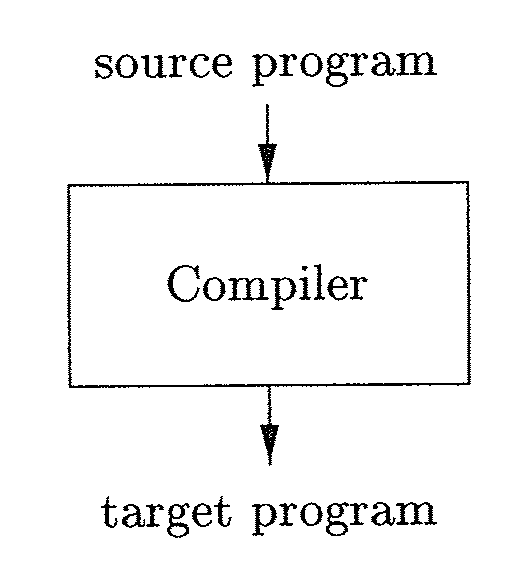
\includegraphics[width=0.8\textwidth]{images/dragon-compiler}
        \caption{Działanie kompilatora \cite{Dragon}}
    \end{figure}
\end{minipage}
};%
%
\tikzoverlay (n1) at (5cm,0cm) {%
\begin{minipage}{0.5\textwidth}%
\begin{block}{}%
\begin{lstlisting}[language=Haskell,basicstyle=\ttfamily,keywordstyle=\color{alerted text.fg}]
main :: IO ()
main = do
    print "Hello world"
\end{lstlisting}
\end{block}
\end{minipage}
};%
%
\tikzoverlay (n2) at (5cm,-3cm) {%
\begin{minipage}{0.5\textwidth}%
\begin{block}{}%
\begin{lstlisting}[basicstyle=\tiny\ttfamily]
001 000 002 000 000 000 000 000 110 145
154 154 157 040 167 157 162 154 144 000
000 000 000 000 116 157 156 124 145 162
155 151 156 141 164 151 157 156 000 000
\end{lstlisting}
\end{block}
\end{minipage}
};%
%
\begin{tikzpicture}[remember picture, overlay]
  \path [line width=0.2cm,->] (7.8cm,-2.2cm) edge (7.8cm,-3.5cm);
\end{tikzpicture}
\end{frame}

\begin{frame}[c]{\currentname}
    \begin{multicols}{2}
    \begin{figure}[H]
        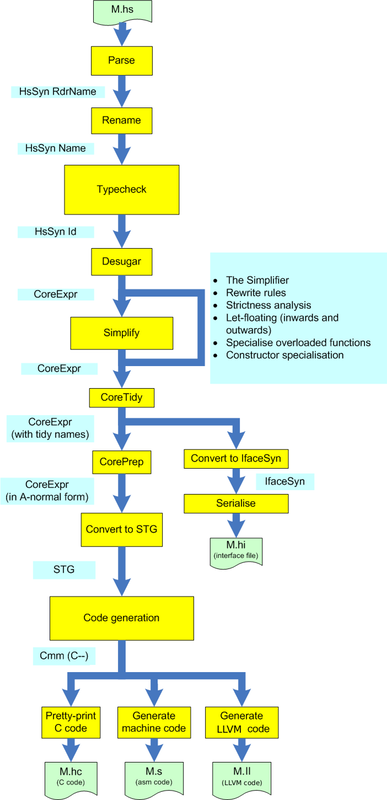
\includegraphics[width=0.2\textwidth]{images/aosa-compiler}
        \caption{Schemat GHC \cite{AOSA}}
    \end{figure}
    \begin{figure}[H]
        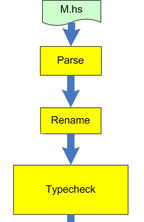
\includegraphics[width=0.27\textwidth]{images/aosa-compiler-cut}
        \caption{Fragment schematu \cite{AOSA}}
    \end{figure}
    \end{multicols}
\end{frame}

\subsection{Type checker} %%%
\begin{frame}[c]{\currentname}
\begin{figure}[H]       
    \centering
    \begin{tikzpicture}[remember picture, overlay]
        \filldraw[fill=yellow, draw=black, fill opacity=0.5] (-5, -3) rectangle (5, 2);
        \filldraw[fill=green, draw=black, fill opacity=0.5] (1.0, -0.8) circle [x radius=3, y radius=2];
        \filldraw[fill=cyan, draw=black, fill opacity=0.5] (-1.0, -0.3) circle [x radius=3, y radius=2];
        \node[draw=black,fill=white,align=center,text width=4cm] at (1.5,-2) {Programy akceptowane przez type checker};
        \node[draw=black,fill=white,align=center] at (-2,1) {Poprawne programy};
        \node[align=center] at (0,-3.3) {Wszystkie programy};
    \end{tikzpicture}
\end{figure}
\end{frame}

\subsection{Problematyka i zakres pracy} %%%
\begin{tframe}{\currentname}
    \begin{itemize}
        \item Dziedziną pracy jest informatyka, tworzenie kompilatorów. 
        
        \item Przedmiotem pracy jest usprawnienie obecnych mechanizmów programowania z użyciem typów w kompilatorze GHC.
         
        \item Type checker to obecnie największy i aktywnie rozwijany komponent GHC\cite{AOSA}. Liczba poprawek i usprawnień czekających na wykonanie jest bardzo duża. 
    \end{itemize}
\end{tframe}

\subsection{Cele pracy} %%%
\begin{tframe}{\currentname}
    \begin{itemize}
        \item Naprawienie błędów i dodanie nowych funkcji do kompilatora GHC, w częściach związanych z programowaniem z użyciem typów.
        \item Zgłoszenie tych rozwiązań i doprowadzenie do ich akceptacji przez deweloperów GHC, by znalazły się w następnej wersji kompilatora. 
    \end{itemize}

    
\end{tframe}

\subsection{Układ pracy} %%%
\begin{tframe}{\currentname} %lub {frame}[t,allowframebreaks] i bez multicols
    \begin{multicols}{2}
        \small
        \tableofcontents
    \end{multicols}
\end{tframe}


\section{Programowanie z użyciem typów} %%%%%%
\subsection{Rodziny typów} %%%
\begin{frame}[t,fragile]{\currentname}
\begin{block}{Zwykła funkcja}
\begin{lstlisting}[language=Haskell,basicstyle=\tiny\ttfamily,keywordstyle=\color{alerted text.fg}]
fib :: Int -> Int
fib 0 = 1
fib 1 = 1
fib n = fib (n - 1) + fib (n - 2)
\end{lstlisting}
\end{block}
\begin{block}{Funkcja na poziomie typów}
\begin{lstlisting}[language=Haskell,basicstyle=\tiny\ttfamily,keywordstyle=\color{alerted text.fg}]
type family Swap a where
    Swap Int = Bool
    Swap Bool = Int
    Swap a = a
\end{lstlisting}
\begin{lstlisting}[language=Haskell,basicstyle=\tiny\ttfamily,keywordstyle=\color{alerted text.fg}]
number :: Swap Bool  -- czyli Int
number = 100
\end{lstlisting}
\end{block}
\end{frame}

\subsection{Częściowe sygnatury typów} %%%
\begin{frame}[t,fragile]{\currentname}
\begin{multicols}{2}
\begin{minipage}{0.4\textwidth}
\begin{block}{}
\begin{lstlisting}[language=Haskell,basicstyle=\tiny\ttfamily,keywordstyle=\color{alerted text.fg}]
add :: Int -> Int -> Int
add x y = x + y
\end{lstlisting}
\end{block}
\end{minipage}
\begin{minipage}{0.4\textwidth}
\begin{block}{}
\begin{lstlisting}[language=Haskell,basicstyle=\tiny\ttfamily,keywordstyle=\color{alerted text.fg}]
--brak sygnatury 
add x y = x + y
\end{lstlisting}
\end{block}
\end{minipage}
\end{multicols}

Częściowa sygnatura z wildcardem '\_a':
\begin{minipage}{1.0\textwidth}
\begin{block}{}
\begin{lstlisting}[language=Haskell,basicstyle=\tiny\ttfamily,keywordstyle=\color{alerted text.fg}]
add :: Int -> _a -> Int
add x y = x + y
\end{lstlisting}
\end{block}
\end{minipage}
\begin{minipage}{1.0\textwidth}
\begin{block}{}
\begin{lstlisting}[language=Haskell,basicstyle=\tiny\ttfamily,keywordstyle=\color{alerted text.fg}]
- Found type wildcard '_a' standing for 'Int'
- In the type signature:
    add :: Int -> _a -> Int
\end{lstlisting}
\end{block}
\end{minipage}
\end{frame}

\section{Technologie i narzędzia wykorzystane w pracy nad GHC} %%%%%%

\subsection{Technologie wykorzystane w pracy nad GHC} %%%
\begin{tframe}{\currentname}
    \begin{figure}
        
\includegraphics[width=0.3\textwidth]{images/icons/Haskell}
        \caption{Logo języka Haskell}
    \end{figure}
\end{tframe}

\subsection{Narzędzia wykorzystane w pracy nad GHC} %%%
\begin{tframe}{\currentname}
    \begin{figure}[H]
    \centering
    \begin{tabu}{cc}
            
\includegraphics[width=0.2\textwidth]{images/icons/Git} &
            
\includegraphics[width=0.10\textwidth]{images/icons/Phabricator}
            \\[3pt]
            \shortstack{Rysunek: Logo systemu\\kontroli wersji Git} & \shortstack{Rysunek: Logo zestawu narzędzi\\ do pracy grupowej Phabricator}
            \\[7pt]
            
\includegraphics[width=0.25\textwidth]{images/icons/Trac} &
            
\includegraphics[width=0.3\textwidth]{images/icons/IntelliJIDEA}
            \\[1pt]
            \shortstack{Rysunek: Logo systemu do\\ zarządzania projektami Trac} & \shortstack{Rysunek: Logo IDE\\ IntelliJ IDEA}
    \end{tabu}
    \end{figure}
\end{tframe}


\section{Usprawnienia dokonane w kompilatorze} %%%%%%

\subsection{Procedura dokonywania zmian w kodzie} %%%
\begin{tframe}{\currentname\cite{wiki}}
    \begin{itemize}
        \item Odnalezienie zgłoszenia w systemie Trac i zostanie jego właścicielem.
        \item Dodanie testu sprawdzającego zamierzone efekty. 
        \item Zaimplementowanie usprawnienia.
        \item Zgłoszenie patcha w systemie Phabricator, gdzie przejdzie on code review i automatyczną weryfikację przez testy.
        \item Zamknięcie zgłoszenia w systemie Trac.
    \end{itemize}
\end{tframe}

\subsection{Zgłoszenie 10839} %%%
\begin{frame}[t,fragile]{\currentname}
\framesubtitle{Consistent pretty-printing of type families}
\small
Błędy generowane przed zmianami.
\begin{block}{}
\begin{lstlisting}[language=Haskell,basicstyle=\tiny\ttfamily]
Conflicting family instance declarations:
  F a -- Defined at Ex1.hs:6:15
  F a -- Defined at Ex1.hs:7:15
\end{lstlisting}
\end{block}
\begin{block}{}
\begin{lstlisting}[language=Haskell,basicstyle=\tiny\ttfamily]
...
In the RHS of type family equation:
forall (k :: BOX) (a :: k) (b :: k). Gc a b = Int
\end{lstlisting}
\end{block}
\begin{block}{}
\begin{lstlisting}[language=Haskell,basicstyle=\tiny\ttfamily]
Overlapped type family instance equation:
  F a = Int
\end{lstlisting}
\end{block}
\end{frame}

\begin{frame}[t,fragile]{\currentname}
\framesubtitle{Consistent pretty-printing of type families}
Błędy generowane po zmianach.
\begin{block}{}
\begin{lstlisting}[language=Haskell,basicstyle=\tiny\ttfamily]
Conflicting family instance declarations:
  F a = a -- Defined at Ex1.hs:6:15
  F a = Int -- Defined at Ex1.hs:7:15
\end{lstlisting}
\end{block}
\begin{block}{}
\begin{lstlisting}[language=Haskell,basicstyle=\tiny\ttfamily]
...
In the type family equation:
  forall k (a :: k) (b :: k). Gc a b = Int -- Defined at Ex3.hs:6:5
\end{lstlisting}
\end{block}
\begin{block}{}
\begin{lstlisting}[language=Haskell,basicstyle=\tiny\ttfamily]
Type family instance equation is overlapped:
  F a = Int -- Defined at Ex2.hs:7:5
\end{lstlisting}
\end{block}
\end{frame}


\subsection{Zgłoszenie 10982} %%%
\begin{frame}[t,fragile]{\currentname}
    \framesubtitle{Warn about unused pattern variables in type families}
\small

Fragment kodu i ostrzeżenie generowane z flagą \emph{-fwarn-unused-matches}.
\begin{block}{}
\begin{lstlisting}[language=Haskell,basicstyle=\tiny\ttfamily]
type family F a b
type instance F a b = a
\end{lstlisting}
\end{block}

\begin{block}{}
\begin{lstlisting}[language=Haskell,basicstyle=\tiny\ttfamily]
Ex5.hs:6:17: warning: Defined but not used: type variable 'b'
\end{lstlisting}
\end{block}

Poprzedzenie lub zastąpienie nazwy podkreślnikiem ucisza kompilator.
\begin{block}{}
\begin{lstlisting}[language=Haskell,basicstyle=\tiny\ttfamily]
type family F a b
type instance F a _b = a
\end{lstlisting}
\end{block}
\end{frame}

\subsection{Zgłoszenie 11098} %%%
\begin{frame}[t,fragile]{\currentname}
    \framesubtitle{PartialTypeSignatures mishandles type variables that begin with an underscore}

Poprawne programy wywoływały błąd kompilacji po uaktywnieniu rozszerzenia NamedWildCards.    
\begin{block}{}
\begin{lstlisting}[language=Haskell,basicstyle=\tiny\ttfamily]
data A a _b = ACon a a 
-- "Unexpected type '_b' In the data declaration for 'A'"
\end{lstlisting}
\end{block}

\begin{block}{}
\begin{lstlisting}[language=Haskell,basicstyle=\tiny\ttfamily]
type family D a b where 
  D _a b = _a -> _a
-- "Wildcard '_a' not allowed in a type pattern of family instance for 'D'"
\end{lstlisting}
\end{block}
\end{frame}

\section{Podsumowanie} %%%%%%

\subsection{Wyniki} %%%
\begin{tframe}{\currentname}
Moja praca doprowadziła do rozwiązania i zamknięcia trzech zgłoszeń w systemie Trac GHC.

\hfill \break
Zmiany, które są wynikiem mojej pracy, to:
    \begin{itemize}
        \item Ujednolicenie wyświetlania rodzin typów.
        \item Generowanie ostrzeżeń o nieużywanych zmiennych typów.
        \item Rozszerzenie NamedWildCards nie powoduje błędów kompilacji.
    \end{itemize}

\end{tframe}

\subsection{Perspektywy rozwoju} %%%
\begin{tframe}{\currentname}
    \begin{itemize}
        \item Zrealizowanie większego, trudniejszego projektu w GHC. Na liście zgłoszeń w Tracu jest wiele pomysłów. 
        \item Praca nad innymi częściami kompilatora: optymalizacje, generator kodu.
    \end{itemize}
\end{tframe}

\section{Bibliografia} %%%
\begin{tframe}{\currentname}
    \begin{thebibliography}{9}
        \small

        \bibitem{TAPL} Benjamin C. Pierce. \emph{Types and Programming Languages}. The MIT Press, 2002. ISBN-10: 0-262-16209-8

        \bibitem{Dragon} Aho, Lam, Sethi, Ullman. \emph{Compilers: Principles, Techniques, and Tools}. Wyd. 2. Harlow: Pearson Education, Inc, 2006. ISBN-10 1-292-02434-8

        \bibitem{AOSA} Amy Brown, Greg Wilson. \emph{The Architecture Of Open Source Applications, Volume II}.  lulu.com, 2008. ISBN-10: 1-105-57181-5

        \bibitem{SLPJ} Simon Peyton Jones. \emph{The Implementation of Functional Programming Languages}. Prentice Hall, 1987. ISBN-10: 0-13-453325-9

        \bibitem{wiki} \emph{https://ghc.haskell.org/trac/ghc/wiki/} (stan na dzień 2015-12-17)

        %\bibitem{proglang} \emph{https://class.coursera.org/proglang-003} (stan na dzień 2015-05-03)

        %\bibitem{automata} \emph{https://class.coursera.org/automata-003} (stan na dzień 2015-05-03)

    \end{thebibliography}
\end{tframe}


\end{document}
